\documentclass{standalone}
\usepackage{tikz}
\usetikzlibrary{patterns, positioning}
\usepackage[sfdefault]{ClearSans} %% option 'sfdefault' activates Clear Sans as the default text font
\usepackage[T1]{fontenc}

\begin{document}
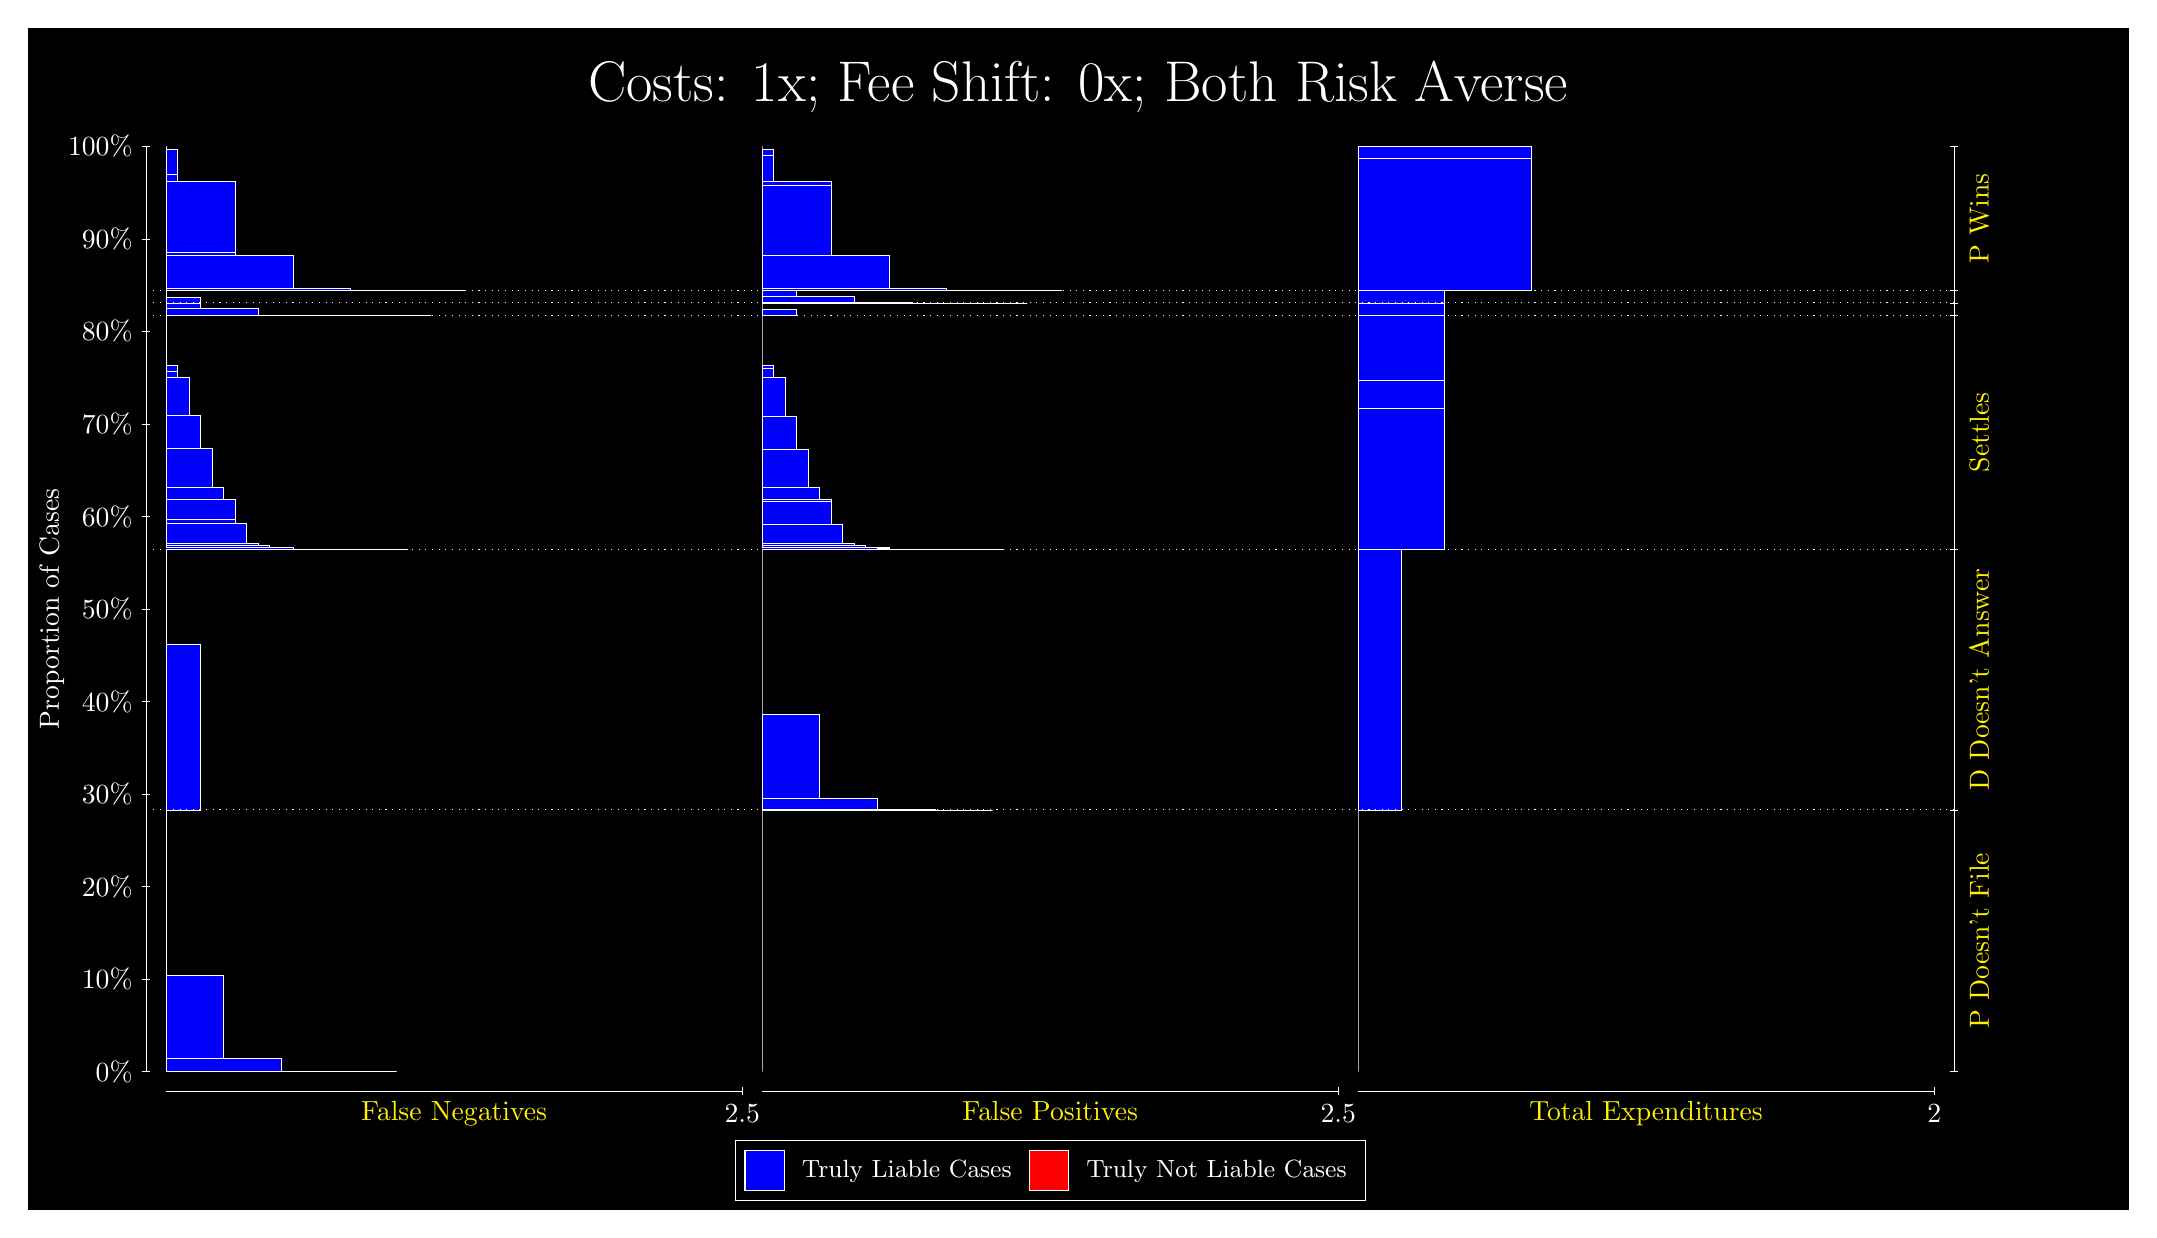
\begin{tikzpicture}
\draw[fill=black] (0,0) rectangle (26.667,15);
\draw[text=white] (0,13.5) rectangle (26.667,15) node[midway] {\huge Costs: 1x; Fee Shift: 0x; Both Risk Averse};
\draw[white, very thin] (1.5,1.75) -- (1.5,13.5);
\node[rotate=90, text=white, anchor=center] at (0.3, 7.625) {Proportion of Cases};
\draw[white, very thin] (1.45,1.75) -- (1.55,1.75);
\node[text=white, anchor=east] at (1.45, 1.75) {0\%};
\draw[white, very thin] (1.45,2.925) -- (1.55,2.925);
\node[text=white, anchor=east] at (1.45, 2.925) {10\%};
\draw[white, very thin] (1.45,4.1) -- (1.55,4.1);
\node[text=white, anchor=east] at (1.45, 4.1) {20\%};
\draw[white, very thin] (1.45,5.275) -- (1.55,5.275);
\node[text=white, anchor=east] at (1.45, 5.275) {30\%};
\draw[white, very thin] (1.45,6.45) -- (1.55,6.45);
\node[text=white, anchor=east] at (1.45, 6.45) {40\%};
\draw[white, very thin] (1.45,7.625) -- (1.55,7.625);
\node[text=white, anchor=east] at (1.45, 7.625) {50\%};
\draw[white, very thin] (1.45,8.8) -- (1.55,8.8);
\node[text=white, anchor=east] at (1.45, 8.8) {60\%};
\draw[white, very thin] (1.45,9.975) -- (1.55,9.975);
\node[text=white, anchor=east] at (1.45, 9.975) {70\%};
\draw[white, very thin] (1.45,11.15) -- (1.55,11.15);
\node[text=white, anchor=east] at (1.45, 11.15) {80\%};
\draw[white, very thin] (1.45,12.325) -- (1.55,12.325);
\node[text=white, anchor=east] at (1.45, 12.325) {90\%};
\draw[white, very thin] (1.45,13.5) -- (1.55,13.5);
\node[text=white, anchor=east] at (1.45, 13.5) {100\%};

\draw[white, very thin] (24.457,1.75) -- (24.457,13.5);
\draw[white, very thin] (24.407,1.75) -- (24.507,1.75);
\node[anchor=west] at (24.407, 1.75) {};
\draw[white, very thin] (24.407,5.0742) -- (24.507,5.0742);
\node[anchor=west] at (24.407, 5.0742) {};
\draw[white, very thin] (24.407,8.3808) -- (24.507,8.3808);
\node[anchor=west] at (24.407, 8.3808) {};
\draw[white, very thin] (24.407,11.356) -- (24.507,11.356);
\node[anchor=west] at (24.407, 11.356) {};
\draw[white, very thin] (24.407,11.513) -- (24.507,11.513);
\node[anchor=west] at (24.407, 11.513) {};
\draw[white, very thin] (24.407,11.671) -- (24.507,11.671);
\node[anchor=west] at (24.407, 11.671) {};
\draw[white, very thin] (24.407,13.5) -- (24.507,13.5);
\node[anchor=west] at (24.407, 13.5) {};

\draw[white, very thin, fill=blue] (1.75,1.75) rectangle (4.6775,1.75);
\draw[white, very thin, fill=blue] (1.75,1.75) rectangle (3.9457,1.7514);
\draw[white, very thin, fill=blue] (1.75,1.7514) rectangle (3.2138,1.9141);
\draw[white, very thin, fill=blue] (1.75,1.9141) rectangle (2.4819,2.9777);
\draw[white, very thin, fill=red] (1.75,2.9777) rectangle (1.75,2.9777);
\draw[white, very thin, fill=blue] (1.75,2.9777) rectangle (1.75,5.0742);
\draw[white, very thin, fill=blue] (1.75,5.0742) rectangle (2.1891,7.171);
\draw[white, very thin, fill=red] (1.75,7.171) rectangle (1.75,7.171);
\draw[white, very thin, fill=blue] (1.75,7.171) rectangle (1.75,8.3808);
\draw[white, very thin, fill=blue] (1.75,8.3808) rectangle (4.8239,8.3808);
\draw[white, very thin, fill=blue] (1.75,8.3808) rectangle (4.2384,8.3808);
\draw[white, very thin, fill=blue] (1.75,8.3808) rectangle (4.092,8.3808);
\draw[white, very thin, fill=blue] (1.75,8.3808) rectangle (3.9457,8.3808);
\draw[white, very thin, fill=blue] (1.75,8.3808) rectangle (3.6529,8.3808);
\draw[white, very thin, fill=blue] (1.75,8.3808) rectangle (3.5065,8.3875);
\draw[white, very thin, fill=blue] (1.75,8.3875) rectangle (3.3602,8.4019);
\draw[white, very thin, fill=blue] (1.75,8.4019) rectangle (3.2138,8.4024);
\draw[white, very thin, fill=blue] (1.75,8.4024) rectangle (3.0674,8.4305);
\draw[white, very thin, fill=blue] (1.75,8.4305) rectangle (2.921,8.459);
\draw[white, very thin, fill=blue] (1.75,8.459) rectangle (2.7746,8.7087);
\draw[white, very thin, fill=blue] (1.75,8.7087) rectangle (2.6283,8.7647);
\draw[white, very thin, fill=blue] (1.75,8.7647) rectangle (2.6283,9.0236);
\draw[white, very thin, fill=blue] (1.75,9.0236) rectangle (2.4819,9.1715);
\draw[white, very thin, fill=blue] (1.75,9.1715) rectangle (2.3355,9.6592);
\draw[white, very thin, fill=blue] (1.75,9.6592) rectangle (2.1891,10.088);
\draw[white, very thin, fill=blue] (1.75,10.088) rectangle (2.0428,10.573);
\draw[white, very thin, fill=blue] (1.75,10.573) rectangle (1.8964,10.637);
\draw[white, very thin, fill=blue] (1.75,10.637) rectangle (1.8964,10.721);
\draw[white, very thin, fill=blue] (1.75,10.721) rectangle (1.75,10.746);
\draw[white, very thin, fill=red] (1.75,10.746) rectangle (1.75,10.746);
\draw[white, very thin, fill=blue] (1.75,10.746) rectangle (1.75,11.356);
\draw[white, very thin, fill=blue] (1.75,11.356) rectangle (5.1167,11.356);
\draw[white, very thin, fill=blue] (1.75,11.356) rectangle (4.3848,11.356);
\draw[white, very thin, fill=blue] (1.75,11.356) rectangle (3.6529,11.357);
\draw[white, very thin, fill=blue] (1.75,11.357) rectangle (2.921,11.437);
\draw[white, very thin, fill=blue] (1.75,11.437) rectangle (2.1891,11.513);
\draw[white, very thin, fill=red] (1.75,11.513) rectangle (1.75,11.513);
\draw[white, very thin, fill=blue] (1.75,11.513) rectangle (2.1891,11.589);
\draw[white, very thin, fill=red] (1.75,11.589) rectangle (1.75,11.589);
\draw[white, very thin, fill=blue] (1.75,11.589) rectangle (1.75,11.671);
\draw[white, very thin, fill=blue] (1.75,11.671) rectangle (5.5558,11.671);
\draw[white, very thin, fill=blue] (1.75,11.671) rectangle (4.8239,11.671);
\draw[white, very thin, fill=blue] (1.75,11.671) rectangle (4.092,11.703);
\draw[white, very thin, fill=blue] (1.75,11.703) rectangle (3.3602,12.117);
\draw[white, very thin, fill=blue] (1.75,12.117) rectangle (2.6283,12.16);
\draw[white, very thin, fill=blue] (1.75,12.16) rectangle (2.6283,13.053);
\draw[white, very thin, fill=blue] (1.75,13.053) rectangle (1.8964,13.141);
\draw[white, very thin, fill=blue] (1.75,13.141) rectangle (1.8964,13.468);
\draw[white, very thin, fill=red] (1.75,13.468) rectangle (1.75,13.468);
\draw[white, very thin, fill=blue] (1.75,13.468) rectangle (1.75,13.5);
\draw[white, very thin, fill=red] (9.3189,1.75) rectangle (9.3189,1.75);
\draw[white, very thin, fill=blue] (9.3189,1.75) rectangle (9.3189,5.0742);
\draw[white, very thin, fill=red] (9.3189,5.0742) rectangle (12.246,5.0742);
\draw[white, very thin, fill=blue] (9.3189,5.0742) rectangle (12.246,5.0742);
\draw[white, very thin, fill=blue] (9.3189,5.0742) rectangle (11.515,5.0747);
\draw[white, very thin, fill=blue] (9.3189,5.0747) rectangle (10.783,5.2196);
\draw[white, very thin, fill=blue] (9.3189,5.2196) rectangle (10.051,6.2839);
\draw[white, very thin, fill=blue] (9.3189,6.2839) rectangle (9.3189,8.3808);
\draw[white, very thin, fill=red] (9.3189,8.3808) rectangle (12.393,8.3808);
\draw[white, very thin, fill=blue] (9.3189,8.3808) rectangle (12.393,8.3808);
\draw[white, very thin, fill=red] (9.3189,8.3808) rectangle (11.807,8.3808);
\draw[white, very thin, fill=blue] (9.3189,8.3808) rectangle (11.807,8.3808);
\draw[white, very thin, fill=blue] (9.3189,8.3808) rectangle (11.661,8.3808);
\draw[white, very thin, fill=red] (9.3189,8.3808) rectangle (11.515,8.3808);
\draw[white, very thin, fill=blue] (9.3189,8.3808) rectangle (11.515,8.3808);
\draw[white, very thin, fill=red] (9.3189,8.3808) rectangle (11.222,8.3808);
\draw[white, very thin, fill=blue] (9.3189,8.3808) rectangle (11.222,8.3808);
\draw[white, very thin, fill=blue] (9.3189,8.3808) rectangle (11.075,8.3875);
\draw[white, very thin, fill=red] (9.3189,8.3875) rectangle (10.929,8.3875);
\draw[white, very thin, fill=blue] (9.3189,8.3875) rectangle (10.929,8.4015);
\draw[white, very thin, fill=red] (9.3189,8.4015) rectangle (10.929,8.4015);
\draw[white, very thin, fill=blue] (9.3189,8.4015) rectangle (10.929,8.4016);
\draw[white, very thin, fill=blue] (9.3189,8.4016) rectangle (10.783,8.402);
\draw[white, very thin, fill=red] (9.3189,8.402) rectangle (10.636,8.402);
\draw[white, very thin, fill=blue] (9.3189,8.402) rectangle (10.636,8.4299);
\draw[white, very thin, fill=blue] (9.3189,8.4299) rectangle (10.49,8.456);
\draw[white, very thin, fill=blue] (9.3189,8.456) rectangle (10.344,8.705);
\draw[white, very thin, fill=blue] (9.3189,8.705) rectangle (10.197,8.9905);
\draw[white, very thin, fill=blue] (9.3189,8.9905) rectangle (10.197,9.0148);
\draw[white, very thin, fill=red] (9.3189,9.0148) rectangle (10.051,9.0148);
\draw[white, very thin, fill=blue] (9.3189,9.0148) rectangle (10.051,9.1636);
\draw[white, very thin, fill=blue] (9.3189,9.1636) rectangle (9.9044,9.648);
\draw[white, very thin, fill=blue] (9.3189,9.648) rectangle (9.758,10.077);
\draw[white, very thin, fill=blue] (9.3189,10.077) rectangle (9.6116,10.565);
\draw[white, very thin, fill=blue] (9.3189,10.565) rectangle (9.4652,10.68);
\draw[white, very thin, fill=blue] (9.3189,10.68) rectangle (9.4652,10.713);
\draw[white, very thin, fill=blue] (9.3189,10.713) rectangle (9.3189,11.356);
\draw[white, very thin, fill=red] (9.3189,11.356) rectangle (9.758,11.356);
\draw[white, very thin, fill=blue] (9.3189,11.356) rectangle (9.758,11.432);
\draw[white, very thin, fill=blue] (9.3189,11.432) rectangle (9.3189,11.513);
\draw[white, very thin, fill=red] (9.3189,11.513) rectangle (12.686,11.513);
\draw[white, very thin, fill=blue] (9.3189,11.513) rectangle (12.686,11.513);
\draw[white, very thin, fill=blue] (9.3189,11.513) rectangle (11.954,11.513);
\draw[white, very thin, fill=blue] (9.3189,11.513) rectangle (11.222,11.515);
\draw[white, very thin, fill=blue] (9.3189,11.515) rectangle (10.49,11.595);
\draw[white, very thin, fill=blue] (9.3189,11.595) rectangle (9.758,11.671);
\draw[white, very thin, fill=red] (9.3189,11.671) rectangle (13.125,11.671);
\draw[white, very thin, fill=blue] (9.3189,11.671) rectangle (13.125,11.671);
\draw[white, very thin, fill=red] (9.3189,11.671) rectangle (12.393,11.671);
\draw[white, very thin, fill=blue] (9.3189,11.671) rectangle (12.393,11.671);
\draw[white, very thin, fill=red] (9.3189,11.671) rectangle (11.661,11.671);
\draw[white, very thin, fill=blue] (9.3189,11.671) rectangle (11.661,11.703);
\draw[white, very thin, fill=red] (9.3189,11.703) rectangle (10.929,11.703);
\draw[white, very thin, fill=blue] (9.3189,11.703) rectangle (10.929,12.117);
\draw[white, very thin, fill=blue] (9.3189,12.117) rectangle (10.197,13.011);
\draw[white, very thin, fill=red] (9.3189,13.011) rectangle (10.197,13.011);
\draw[white, very thin, fill=blue] (9.3189,13.011) rectangle (10.197,13.053);
\draw[white, very thin, fill=blue] (9.3189,13.053) rectangle (9.4652,13.38);
\draw[white, very thin, fill=blue] (9.3189,13.38) rectangle (9.4652,13.468);
\draw[white, very thin, fill=blue] (9.3189,13.468) rectangle (9.3189,13.5);
\draw[white, very thin, fill=red] (16.888,1.75) rectangle (16.888,1.75);
\draw[white, very thin, fill=blue] (16.888,1.75) rectangle (16.888,5.0742);
\draw[white, very thin, fill=red] (16.888,5.0742) rectangle (17.437,5.0742);
\draw[white, very thin, fill=blue] (16.888,5.0742) rectangle (17.437,8.3808);
\draw[white, very thin, fill=red] (16.888,8.3808) rectangle (17.986,8.3808);
\draw[white, very thin, fill=blue] (16.888,8.3808) rectangle (17.986,10.172);
\draw[white, very thin, fill=red] (16.888,10.172) rectangle (17.986,10.172);
\draw[white, very thin, fill=blue] (16.888,10.172) rectangle (17.986,10.529);
\draw[white, very thin, fill=red] (16.888,10.529) rectangle (17.986,10.529);
\draw[white, very thin, fill=blue] (16.888,10.529) rectangle (17.986,11.356);
\draw[white, very thin, fill=red] (16.888,11.356) rectangle (17.986,11.356);
\draw[white, very thin, fill=blue] (16.888,11.356) rectangle (17.986,11.513);
\draw[white, very thin, fill=red] (16.888,11.513) rectangle (17.986,11.513);
\draw[white, very thin, fill=blue] (16.888,11.513) rectangle (17.986,11.671);
\draw[white, very thin, fill=red] (16.888,11.671) rectangle (19.083,11.671);
\draw[white, very thin, fill=blue] (16.888,11.671) rectangle (19.083,13.348);
\draw[white, very thin, fill=red] (16.888,13.348) rectangle (19.083,13.348);
\draw[white, very thin, fill=blue] (16.888,13.348) rectangle (19.083,13.5);
\draw[white, dotted] (1.5,5.0742) -- (24.457,5.0742);
\draw[white, dotted] (1.5,8.3808) -- (24.457,8.3808);
\draw[white, dotted] (1.5,11.356) -- (24.457,11.356);
\draw[white, dotted] (1.5,11.513) -- (24.457,11.513);
\draw[white, dotted] (1.5,11.671) -- (24.457,11.671);
\draw[white, very thin] (1.75,1.5) -- (9.0689,1.5);
\node[text=yellow, anchor=north] at (5.4094, 1.5) {False Negatives};
\draw[white, very thin] (9.0689,1.45) -- (9.0689,1.55);
\node[text=white, anchor=north] at (9.0689, 1.45) {2.5};

\draw[white, very thin] (9.3189,1.5) -- (16.638,1.5);
\node[text=yellow, anchor=north] at (12.978, 1.5) {False Positives};
\draw[white, very thin] (16.638,1.45) -- (16.638,1.55);
\node[text=white, anchor=north] at (16.638, 1.45) {2.5};

\draw[white, very thin] (16.888,1.5) -- (24.207,1.5);
\node[text=yellow, anchor=north] at (20.547, 1.5) {Total Expenditures};
\draw[white, very thin] (24.207,1.45) -- (24.207,1.55);
\node[text=white, anchor=north] at (24.207, 1.45) {2};

\node[text=yellow, centered, rotate=90] at (24.777, 3.4121) {P Doesn't File};
\node[text=yellow, centered, rotate=90] at (24.777, 6.7275) {D Doesn't Answer};
\node[text=yellow, centered, rotate=90] at (24.777, 9.8682) {Settles};


\node[text=yellow, centered, rotate=90] at (24.777, 12.585) {P Wins};

\draw (12.978300999999998,1.5) node[draw=none] (baseCoordinate) {};
\begin{scope}[align=center]
        \matrix[scale=0.5, draw=white, below=0.5cm of baseCoordinate, nodes={draw}, column sep=0.1cm]{
            \node[rectangle, draw, minimum width=0.5cm, minimum height=0.5cm, fill=blue] {}; &
            \node[draw=none, font=\small, text=white] (B) {Truly Liable Cases}; &
            \node[rectangle, draw, minimum width=0.5cm, minimum height=0.5cm, fill=red] {}; &
            \node[draw=none, font=\small, text=white] (B) {Truly Not Liable Cases}; \\
            };
\end{scope}

\end{tikzpicture}
\end{document}